

In this thesis, we make contributions at the intersection between neural networks and structured matrices.
We build neural networks with structured matrices and develop new algorithms for training neural networks based on certain properties of structured matrices. 
Hereafter, we present some preliminaries on structured matrices that we will use later. 

%%%%%%%%%%%%%%%%%%%%%%%%%%%%%%%%%%%%%%%%%%%%%%%%%%%%%%%%%%%%%%%%%%%%%%%%%%%%%%%
\subsection{Toeplitz Matrices}
\label{subsection:ch2-toeplitz_matrices}
%%%%%%%%%%%%%%%%%%%%%%%%%%%%%%%%%%%%%%%%%%%%%%%%%%%%%%%%%%%%%%%%%%%%%%%%%%%%%%%

A Toeplitz matrix, named after Otto Toeplitz, is a matrix in which each descending diagonal from left to right is constant.
Let $P = \{-n+1, \dots, n-1\}$, an $n\times n$ Toeplitz matrix $\Amat$ is fully determined by a two-sided sequence of scalars $\{a_h\}_{h \in P}$ as follows:
\begin{equation}
  \Amat =
  \leftmatrix
    a_0 & a_{1} & a_{2} & \cdots & \cdots & a_{n-1} \\
    a_{-1} & a_0 & a_{1} & \ddots & & \vdots \\
    a_{-2} & a_{-1} & \ddots & \ddots & \ddots & \vdots \\
    \vdots & \ddots & \ddots & \ddots & a_{1} & a_{2} \\
    \vdots & & \ddots & a_{-1} & a_{0} & a_{1} \\
    a_{-n+1} & \cdots & \cdots & a_{-2} & a_{-1} & a_0
  \rightmatrix
\end{equation}
\noindent
Because the Toeplitz matrix $\Amat$ is fully determined by the sequence $\{a_h\}_{h \in P}$, it can be compactly represented in memory using only $2n-1$ values instead of $n^2$.
Toeplitz matrices can also be characterized by noting that the $(k,j)$ entry of $\Amat$, $\leftmat \Amat \rightmat_{j,k}$ is given by
\begin{equation}
  \leftmat \Amat \rightmat_{j,k} = a_{k-j} \enspace.
\end{equation}

A standard tool for manipulating Toeplitz matrices is the use of Fourier analysis.
Let $\{a_h\}_{h \in P}$ be the sequence of coefficients of the Toeplitz matrix $\Amat \in \mathbb{R}^{n\times n}$.
The complex-valued function 
\begin{equation}
  f(\omega) = \sum_{h \in P} a_h e^{\ci h \omega}
\end{equation}
is the \emph{inverse Fourier transforms} of the sequences $\{a_h\}_{h \in P}$ with $\omega \in \mathbb{R}$.
From this function, one can recover the sequence $\{a_h\}_{h \in P}$ using the standard Fourier transform:
\begin{equation}
  a_h = \frac{1}{2\pi} \int_0^{2\pi} e^{-\ci h \omega} f(\omega) d\omega \enspace. 
\end{equation}

From there, similarly to the work done by~\citet{gray2006toeplitz}, we can define an operator $\Tmat$ mapping integrable functions to matrices:
\begin{equation}
  \Tmat_n(g) \triangleq \leftmat\frac{1}{2\pi}\int_{0}^{2\pi}e^{-\ci(i-j)\omega}g(\omega)\,d\omega\rightmat_{i,j\in\{0,\ldots,n-1\}} \enspace.
  \label{equation:ch2-toeplitz_operator}
\end{equation}
\noindent
In the following of this thesis, when it is clear from context, we will write $\Tmat(g)$ instead of $\Tmat_n(g)$.
We can show that if $f$ is the inverse Fourier transform of $\{a_h\}_{h \in P}$, then $\Tmat_n(f)$ is equal to $\Amat$.
\begingroup
\allowdisplaybreaks
  \begin{align}
      \leftmat \Tmat_n(f) \rightmat_{i, j} &= \frac{1}{2\pi} \int_0^{2\pi} e^{-\ci (i-j)\omega} f(\omega) \,d\omega  \\
      &= \frac{1}{2\pi} \int_0^{2\pi} e^{-\ci (i-j) \omega} \sum_{h \in N} a_h e^{\ci h \omega} \,d\omega  \\
      &= \frac{1}{2\pi} \int_0^{2\pi} \sum_{h \in N} a_h e^{\ci (j - i + h) \omega} \,d\omega  \\
      &= \sum_{h \in N} a_h \frac{1}{2\pi} \int_0^{2\pi} e^{\ci (j - i + h) \omega} \,d\omega 
      = a_{j-i} .
  \end{align}
\endgroup
Because:
\begin{equation}
  \frac{1}{2\pi} \int_0^{2\pi} e^{\ci k \omega} \,d\omega = 
  \begin{cases}
    1 \quad \text{if}\ k = 0, \\
    0 \quad \text{if}\ k\ \text{is a non-zero integer number.}
  \end{cases}
\end{equation}

% Also, if $F$ is the inverse Fourier transform of $\{\Bmat_h\}_{h \in P}$ as defined above, then the integral in \Cref{equation:expression_toeplitz_matrix} is matrix-valued, and thus $\Tmat(F) \in \mathbb{R}^{mn \times mn}$ is the block matrix $\Bmat$.

% The trigonometric polynomial that \emph{generates} the Toeplitz matrix $\Amat$ can be defined as follows:
% \begin{equation}
%   f_{\Amat}(\omega) \triangleq \sum_{h \in N} a_h e^{\ci h \omega}
% \end{equation}
% The function $f_{\Amat}$ is said to be the \emph{generating function} of $\Amat$.
% To recover the Toeplitz matrix from its generating function, we have the following operator:
% \begin{equation}
%   \leftmat \Tmat(f) \rightmat_{i, j} \triangleq \frac{1}{2\pi} \int_0^{2\pi} e^{-\ci (i - j)\omega} f(\omega) \,d\omega .
%   \label{equation:ch2-toeplitz_operator}
% \end{equation}


%%%%%%%%%%%%%%%%%%%%%%%%%%%%%%%%%%%%%%%%%%%%%%%%%%%%%%%%%%%%%%%%%%%%%%%%%%%%%%%
\subsection{Circulant Matrices}
\label{subsection:ch2-circulant_matrices}
%%%%%%%%%%%%%%%%%%%%%%%%%%%%%%%%%%%%%%%%%%%%%%%%%%%%%%%%%%%%%%%%%%%%%%%%%%%%%%%

Circulant matrices are a special case of Toeplitz matrices.
In addition to having constant diagonals, each row of a circulant matrix is a cyclic right shift of the previous one.
% Circulant matrices have been used to efficiently solve linear systems~\cite{golub1996matrix} and years later were used to perform dimensionality reduction~\cite{hinrichs2011johnson,vybiral2011variant}, binary embedding~\cite{yu2014circulant} and kernel approximation~\cite{yu2015compact} in the context of pattern recognition and machine learning.
An $n \times n$ circulant matrix $\Cmat$ is fully determined by a sequence of scalars $\{c_h\}_{h \in [0,n-1]}$ as follows:

\begin{equation}
  \Cmat =
  \leftmatrix
    c_0 & c_{n-1} & c_{n-2} & \cdots & \cdots & c_{1} \\
    c_{1} & c_0 & c_{n-1} & \ddots & & \vdots \\
    c_{2} & c_{1} & \ddots & \ddots & \ddots & \vdots \\
    \vdots & \ddots & \ddots & \ddots & c_{n-1} & c_{n-2} \\
    \vdots & & \ddots & c_{1} & c_{0} & c_{n-1} \\
    c_{n-1} & \cdots & \cdots & c_{2} & c_{1} & c_0
  \rightmatrix
\end{equation}

Because the circulant matrix $\Cmat$ is fully determined by the sequence $\{c_h\}_{h \in [0,n-1]}$, it can be compactly represented in memory using only $n$ values instead of $n^2$.
Circulant matrices can also be characterized by noting that the $(k,j)$ entry of $\Cmat$, $\leftmat \Cmat \rightmat_{j,k}$ is given by
\begin{equation}
  \leftmat \Cmat \rightmat_{j,k} = c_{\left(k-j\right) \mod n} \enspace.
\end{equation}
% We can also denote the sequence $\{c_h\}$ as a vector $\cvec$ such that $\forall i, \cvec_i = c_i$. The circulant matrices can then be expressed with $\Cmat = \circulant(\cvec)$.
Circulant matrices exhibit several interesting properties which are based on the fact that they can be diagonalized by the Discrete Fourier Transform (DFT)~\cite{davis1979circulant}.
First, we define the Fourier Matrix and then, we present an important theorem regarding eigenvalues and eigenvectors of circulant matrices.

\begin{definition}[Fourier Matrix]
  The Fourier matrix of order $n$ is defined as follows:
  \begin{equation}
    \Umat_n = 
    \leftmatrix
      1      & 1           & 1              & \cdots & 1           \\
      1      & z_n       & z_d^2        & \cdots & z_d^{d-1} \\
      1      & z_n^2     & z_d^4        & \cdots & z_d^{2(d-1)} \\
      \vdots & \vdots      & \vdots         &        & \vdots      \\
      1      & z_n^{n-1} & z_d^{2(n-1)} & \cdots & z_d^{(d-1)(d-1)}
    \rightmatrix
  \end{equation}
  where $z_n = e^{-\frac{2\pi\ci}{n}}$ is an $n^{\text{th}}$ root of unity.
  \label{definition:ch2-fourier_matrix}
\end{definition}
\noindent
The matrix-vector product between the Fourier matrix above and a vector is equivalent to apply the Discrete Fourier Transform on the vector.
This matrix-vector product can be efficiently computed with the \emph{Fast Fourier transform} (FFT) algorithm~\cite{cooley1965algorithm}.
The complexity is reduced from from $\bigO(n^2)$ to $\bigO(n \log n)$.

\begin{theorem}[Theorem 3.1 of \citet{gray2006toeplitz}]
  Every $n \times n$ circulant matrix $\Cmat$, has eigenvectors  
  \begin{equation}
    \yvec^{(k)} = \frac{1}{\sqrt{n}} \leftmatrix 1, e^{-\frac{2 \pi \ci k}{n}}, \dots, e^{-\frac{2 \pi \ci k(n-1)}{n}} \rightmatrix^\top
  \end{equation}
  and corresponding eigenvalues
  \begin{equation}
    \psi_k = \sum_{j=0}^{n-1} c_j e^{-\frac{2 \pi \ci}{n} jk}
  \end{equation}
  The circulant matrix $\Cmat$ can be expressed in the form 
  \begin{equation}
    \Cmat = \frac{1}{n} \Umat_n^* \diag(\Umat_n \cvec) \Umat_n
    \label{equation:ch2-diagonalization_circulant_matrix}
  \end{equation}
  where $\cvec$ is vector based of the scalars $\{c_h\}_{h \in [0,n-1]}$.
  In particular all circulant matrices share the same eigenvectors, the same matrix $\Umat_n$ works for all $n \times n$ circulant matrices.
  Also, circulant matrices commute and are closed under sum and product.
  \label{theorem:ch2-diagonalization_circulant_matrix}
\end{theorem}
\noindent
Based on \Cref{theorem:ch2-diagonalization_circulant_matrix} and of the \emph{Fast Fourier transform} (FFT) algorithm the matrix-vector product between a circulant matrix $\Cmat$ and a vector $\xvec$ can be reduced from $\bigO(n^2)$ to $\bigO(n \log n)$. 
If we denote the Fast Fourier transform algorithm by \textbf{FFT} and the inverse by \textbf{IFFT}, the pseudocode for the matrix-product between a circulant matrix and a vector is as follows:
\begin{algorithm}[h]
  \begin{algorithmic}[1]
    \Procedure{input}{$\cvec, \xvec$} \Comment{first column of the circulant matrix $\Cmat$, vector $\xvec$}
      \State $\tilde{\xvec} \gets \textbf{FFT}(\xvec)$
      \State $\tilde{\cvec} \gets \textbf{FFT}(\cvec)$
      \State $\yvec \gets \textbf{IFFT}(\tilde{\xvec} * \tilde{\cvec})$ \Comment{element-wise vector-vector product}
      \State \textbf{return} $\yvec$ \Comment{return the result of the product $\Cmat \xvec$}
    \EndProcedure
  \end{algorithmic}
  \caption{Matrix-vector product with a circulant matrix}
  \label{algorithm:ch2-matrix_vector_product_circulant_matrix}
\end{algorithm}

An important object based on circulant matrices are called \emph{$f$-circulant matrices} and are defined as follows:
\begin{definition}[$f$-circulant matrix]
  Given a vector $\xvec$, the $f$-circulant matrix, $\Zmat_f(\xvec)$, is defined as follows:
  \begin{equation}
    \Zmat_f(\xvec) \triangleq
    \leftmatrix
      \xvec_0 & $f$ \xvec_{n-1} & $f$ \xvec_{n-2} & \cdots & \cdots & $f$ \xvec_{1} \\
      \xvec_{1} & \xvec_0 & $f$ \xvec_{n-1} & \ddots & & \vdots \\
      \xvec_{2} & \xvec_{1} & \ddots & \ddots & \ddots & \vdots \\ 
      \vdots & \ddots & \ddots & \ddots & $f$ \xvec_{n-1} & $f$ \xvec_{n-2} \\
      \vdots & & \ddots & \xvec_{1} & \xvec_{0} & $f$ \xvec_{n-1} \\
      \xvec_{n-1} & \cdots & \cdots & \xvec_{2} & \xvec_{1} & \xvec_0
    \rightmatrix
  \end{equation}
  \label{definition:ch2-f_circulant_matrix}
  \removespace
\end{definition}
\noindent
A $f$-unit-circulant, denoted $\Zmat_f$, is a $f$-circulant matrix defined by the vector $\left(0, 1, \dots, 0 \right)$:
\begin{equation}
  \Zmat_f = \circulant \left(e^{(1)} \right) + (f - 1) \evec^{(0)} \evec^{(n-1)\top}
\end{equation}

Thus, in matrix form, we have:
\begin{equation}
  \Zmat_f = 
    \leftmatrix
      0      & 0      & 0      & \cdots & \cdots & f      \\
      1      & 0      & 0      & \ddots &        & \vdots \\
      0      & 1      & \ddots & \ddots & \ddots & \vdots \\ 
      \vdots & \ddots & \ddots & \ddots & 0      & 0      \\
      \vdots &        & \ddots & 1      & 0      & 0      \\
      0      & \cdots & \cdots & 0      & 1      & 0
    \rightmatrix
\end{equation}

\noindent
As stated by~\citet{sindhwani2015structured}, the $f$-unit-circulant matrix performs a downward shift-and-scale transformation on a vector.
More precisely, the matrix-vector product $\Zmat_f \xvec$ makes a circular shifts on the elements and scale the last element of the vector resulting in $\Zmat_f \xvec = \leftmat f \xvec_{n-1}, \xvec_0, \dots, \xvec_{n-2} \rightmat^\top$. 
$f$-unit-circulant matrix are one of the building block of \emph{Low displacement rank operator} presented in \Cref{subsection:ch3-building_compact_neural_networks_with_structured_matrices}.


% The f-unit-circulant matrix is associated with a basic downward shift-and-scale transformation, i.e.,
% the matrix-vector product Zfv shifts the elements of the column vector v “downwards”, and scales
% and brings the last element vn to the “top”, resulting in [fvn, v1, . . . vn−1] T .
% It has several basic
% algebraic properties (see Proposition 1.1 [1]) that are crucial for the results stated in this section



% the complexity of the matrix-vector product between a circulant matrix $\Cmat$ and a vector $\xvec$ can be reduced from $\bigO(n^2)$ to $\bigO(n \log n)$ with the \emph{Fast Fourier transform} (FFT) algorithm~\cite{cooley1965algorithm}.

% More precisely, the eigenvalues $\psi_k$ of the matrix $\Cmat$ correspond to the discrete Fourier transform of the vector characteristic $\cvec$:
% and the eigenvectors $\yvec^{(k)}$ can be expressed as follows:
% \begin{equation}
%   \yvec^{(k)} = \frac{1}{\sqrt{n}} \leftmatrix 1, e^{-\frac{2 \pi \ci k}{n}}, \dots, e^{-\frac{2 \pi \ci k(n-1)}{n}} \rightmatrix^\top
% \end{equation}
% In matrix form, we can diagonalize the matrix $\Cmat$ as follows:
% \begin{equation}
%   \Cmat = \frac{1}{n} \Umat_n^* \diag(\Umat_n \cvec) \Umat_n
% \end{equation}
% where $\Umat_n = \leftmatrix e^{-\frac{2 \pi \ci jk}{n}} \rightmatrix_{j,k = 0}^{n-1}$ is the DFT matrix and $\cvec$ is vector based of the scalars $\{c_h\}_{h \in \{0, \dots, n-1\}}$.

% The following Theorem summarize the propreties for circulant matrices derived above.



\comment{


%%%%%%%%%%%%%%%%%%%%%%%%%%%%%%%%%%%%%%%%%%%%%%%%%%%%%%%%%%%%%%%%%%%%%%%%%%%%%%%
\subsection{Relationship between Toeplitz and circulant matrices}
\label{subsection:ch2-relationship_between_toeplitz_and_circulant_matrices}
%%%%%%%%%%%%%%%%%%%%%%%%%%%%%%%%%%%%%%%%%%%%%%%%%%%%%%%%%%%%%%%%%%%%%%%%%%%%%%%


This assumption is justified by the work of \citet{gray2006toeplitz,gutierrez2012block} which states that a sequence of block Toeplitz matrices is asymptotically equivalent to a sequence of sequence of block circulant matrices.

The concept of asymptotically equivalent sequences can be illustrated by the following. 
Consider the infinite sequence $\{a_k\}$ and define the corresponding $n \times n$ Toeplitz operator $\Tmat(n) = \leftmat a_{k-j} \rightmat_{k,j = 0}^{n-1}$.
We call \emph{banded}-Toeplitz matrix, a Toeplitz matrix for which it exists an $m$ such that $a_k = 0$, for $|k| > m$.
A $n \times n$ banded-Toeplitz matrix can be represented as follows:
\begin{equation}
  \Tmat(n)  =
  \leftmatrix
    a_0    & a_1    & \cdots   & a_m    &        &        &        &        &        &        \\
    a_{-1} & a_0    & a_1      &        & \ddots &        &        &        &        &        \\
    \vdots & a_{-1} & \ddots   & \ddots &        & \ddots &        & 0      &        &        \\
    a_{-m} &        & \ddots   & \ddots & \ddots &        & a_m    &        &        &        \\ 
           & \ddots &          & \ddots & a_0    & a_1    &        & \ddots &        &        \\
	   &        & \ddots   &        & a_{-1} & \ddots & \ddots &        & \ddots &        \\
	   &        &          & a_{-m} &        & \ddots & \ddots & \ddots &        & a_m    \\
    	   &        & 0        &        & \ddots &        & \ddots & \ddots & a_1    & \vdots \\
           &        &          &        &        & \ddots &        & a_{-1}  & a_0    & a_1   \\  
           &        &          &        &        &        & a_{-m} & \cdots & a_{-1} & a_0    \\ 
  \rightmatrix
\end{equation}
\citet{gray2006toeplitz} has noted that the only difference between a $n \times n$ banded-Toeplitz matrix and a circulant matrix based on the same sequence is the values on the bottom-left and top-right corner of the matrix.
The circulant matrix based on the same sequence $\{a_k\}$ can be represented as follows:
\begin{equation}
  \Cmat(n)  =
  \leftmatrix
    a_0    & a_1    & \cdots   & a_m    &        &        &        & a_{-m} & \cdots & a_{-1} \\
    a_{-1} & a_0    & a_1      &        & \ddots &        &        &        & \ddots & \vdots \\
    \vdots & a_{-1} & \ddots   & \ddots &        & \ddots &        & 0      &        & a_{-m} \\
    a_{-m} &        & \ddots   & \ddots & \ddots &        & a_m    &        &        &        \\ 
           & \ddots &          & \ddots & a_0    & a_1    &        & \ddots &        &        \\
	   &        & \ddots   &        & a_{-1} & \ddots & \ddots &        & \ddots &        \\
	   &        &          & a_{-m} &        & \ddots & \ddots & \ddots &        & a_m    \\
    a_m	   &        & 0        &        & \ddots &        & \ddots & \ddots & a_1    & \vdots \\
    \vdots & \ddots &          &        &        & \ddots &        & a_{-1} & a_0    & a_1    \\  
    a_1    & \cdots & a_m      &        &        &        & a_{-m} & \cdots & a_{-1} & a_0    \\ 
  \rightmatrix
\end{equation}
\noindent
Thus, the greater the difference between $n$ and $m$, the `closer' the banded-Toeplitz matrix will be to the circulant one. 
This concept of closeness between Toeplitz and a circulant matrix have been extensively studied and extended to block Toeplitz and block circulant matrices~\cite{Toeplitz1911,widom1976asymptotic,gazzah2001asymptotic,gray2006toeplitz,gutierrez2008asymptotically,gutierrez2011asymptotically,gutierrez2012block,zhu2017asymptotic,oudin2008asymptotic}.


}



%%%%%%%%%%%%%%%%%%%%%%%%%%%%%%%%%%%%%%%%%%%%%%%%%%%%%%%%%%%%%%%%%%%%%%%%%%%%%%%
\subsection{Block Toeplitz and Block Circulant Matrices}
\label{subsection:ch2-block_toeplitz_and_block_circulant_matrices}
%%%%%%%%%%%%%%%%%%%%%%%%%%%%%%%%%%%%%%%%%%%%%%%%%%%%%%%%%%%%%%%%%%%%%%%%%%%%%%%

We can extend the logic of Toeplitz and circulant matrices to block Toeplitz and block circulant matrices.
A block Toeplitz matrix is a matrix in which each block is repeated identically along diagonals.
Equivalently, a block circulant matrix is a matrix in which each block is repeated identically along diagonals (like block Toeplitz matrices) and each ``row of blocks'' is cyclic right shift of the previous one.
We show that block Toeplitz and block circulant matrices have similar properties that Toeplitz and circulant matrices.

A $nm\times nm$ block circulant matrix $\Amat$ is fully determined by a sequence of blocks $\{\Amat_h\}_{h \in [0,n-1]}$ and where each block $\Amat_h$ is an $m \times m$ matrix.
The circulant matrix $\Amat$ has the following form:
\begin{equation}
  \Amat = \leftmat \Amat_{(k-j) \mod n} \rightmat_{i, j = 0}^{n-1} = 
  \leftmatrix
    \Amat_{0}   & \Amat_{n-1} & \Amat_{n-2} & \cdots    & \cdots      & \Amat_{1}   \\
    \Amat_{1}   & \Amat_{0}   & \Amat_{n-1} & \ddots    &             & \vdots      \\
    \Amat_{2}   & \Amat_{1}   & \ddots      & \ddots    & \ddots      & \vdots      \\ 
    \vdots      & \ddots      & \ddots      & \ddots    & \Amat_{n-1} & \Amat_{n-2} \\
    \vdots      &             & \ddots      & \Amat_{1} & \Amat_{0}   & \Amat_{n-1} \\
    \Amat_{n-1} & \cdots      & \cdots      & \Amat_{2} & \Amat_{1}   & \Amat_{0}
  \rightmatrix
\end{equation}
% \begin{equation}
%   \Amat = \leftmat \Amat_{(k-j) \mod n} \rightmat_{i, j = 0}^{n-1} =
%   \leftmatrix
%     \Amat_{0}   & \Amat_{n-1} & \cdots    & \Amat_{1}   \\
%     \Amat_{1}   & \Amat_{0}   & \ddots    & \vdots      \\
%     \vdots      & \ddots      & \ddots    & \Amat_{n-1} \\
%     \Amat_{n-1} & \cdots      & \Amat_{1} & \Amat_{0}
%   \rightmatrix
% \end{equation}


In a similar way to circulant matrices, block circulant matrices have a relation with the Discrete Fourier Transform.
The next result characterizes this relation:
\begin{theorem}[Lemma 5.1 of \citet{gutierrez2012block}]
  Let $\Amat$ be a $nm\times nm$ block circulant matrix defined by the sequence of blocks $\{\Amat_h\}_{h \in [0,n-1]}$, then:
  \begin{equation}
    \Amat = (\Umat_n \otimes \Imat_n) \diag(\Psi_0, \dots, \Psi_{n-1}) (\Umat_n \otimes \Imat_n)^*
  \end{equation}
  where $\otimes$ is the Kronecker product, $\Umat_n$ is the Fourier matrix of size $n \times n$ and

  \begin{equation}
    \leftmatrix
      \Psi_{0} \\
      \Psi_{1} \\
      \vdots \\
      \Psi_{n-1} \\
    \rightmatrix = 
    \sqrt{n}(\Umat_n \otimes \Imat_n)^* 
    \leftmatrix
      \Amat_{0} \\
      \Amat_{1} \\
      \vdots \\
      \Amat_{n-1} \\
    \rightmatrix
  \end{equation}
  \removespace
\end{theorem}
\noindent
One can remark that when the blocks are of size $1\times1$ \ie, scalar, this theorem coincide with \Cref{equation:ch2-diagonalization_circulant_matrix} of \Cref{theorem:ch2-diagonalization_circulant_matrix}.
Another interesting special case is when the blocks of the block circulant matrix are also circulant, such matrix are called doubly-block circulant matrices.
In this case, we have the following result:

\begin{theorem}[Section 5.5 of \citet{jain1989fundamentals}] 
  The eigenvectors of every $n^2 \times n^2$ doubly-block circulant matrices are the columns of the matrix $\frac{1}{n} \left( \Umat_n \otimes \Umat_n \right)$.
  \label{theorem:ch2-diaginalization_doubly_block_circulant_matrix}
\end{theorem}


In a similar way as Toeplitz matrices, block Toeplitz matrices can be expressed with the Toeplitz operator defined in \Cref{equation:ch2-toeplitz_operator}.
A $nm\times nm$ block Toeplitz matrix $\Bmat$ is fully determined by a two-sided sequence of blocks $\{\Bmat_h\}_{h \in P}$ and where each block $\Bmat_h$ is an $m \times m$ matrix.  
The block Toeplitz matrix $\Bmat$ has the following form:
\begin{equation}
  \Bmat = \leftmat \Bmat_{k-j} \rightmat_{j,k = 0}^{n-1} = 
  \leftmatrix
    \Bmat_{0}    & \Bmat_{1}  & \Bmat_{2} & \cdots     & \cdots     & \Bmat_{n-1} \\
    \Bmat_{-1}   & \Bmat_{0}  & \Bmat_{1} & \ddots     &            & \vdots      \\
    \Bmat_{-2}   & \Bmat_{-1} & \ddots    & \ddots     & \ddots     & \vdots      \\ 
    \vdots       & \ddots     & \ddots    & \ddots     & \Bmat_{1}  & \Bmat_{2}   \\
    \vdots       &            & \ddots    & \Bmat_{-1} & \Bmat_{0}  & \Bmat_{1}   \\
    \Bmat_{-n+1} & \cdots     & \cdots    & \Bmat_{-2} & \Bmat_{-1} & \Bmat_0
  \rightmatrix
\end{equation}
% \begin{equation}
%   \Bmat = \leftmat \Bmat_{k-j} \rightmat_{j,k = 0}^{n-1} = 
%   \leftmatrix
%     \Bmat_{0}    & \Bmat_{1}  & \cdots     & \Bmat_{n-1} \\
%     \Bmat_{-1}   & \Bmat_{0}  & \ddots     & \vdots      \\
%     \vdots       & \ddots     & \ddots     & \Bmat_{1}   \\
%     \Bmat_{-n+1} & \cdots     & \Bmat_{-1} & \Bmat_{0}   \\
%   \rightmatrix
% \end{equation}
\noindent
% The same reasoning can be applied to block Toeplitz matrices.
Instead of being complex-valued, the trigonometric polynomial that \emph{generates} the block Toeplitz $\Bmat$ is matrix-valued and can be defined as follows:
\begin{equation}
  F_{\Bmat}(\omega) \triangleq \sum_{h \in P} \Bmat_h e^{\ci h \omega}
\end{equation}
The function $F_{\Bmat}$ is said to be the \emph{generating function} of $\Bmat$.
To recover the block Toeplitz matrix from its generating function, we use the Toeplitz operator defined in \Cref{equation:ch2-toeplitz_operator}; therefore, we have $\Tmat_n(F_\Bmat) = \Bmat$.

%%%%%%%%%%%%%%%%%%%%%%%%%%%%%%%%%%%%%%%%%%%%%%%%%%%%%%%%%%%%%%%%%%%%%%%%%%%%%%%
\subsection{The Structure of the Convolution Operator}
\label{subsection:ch2-the_structure_of_the_convolution_operator}
%%%%%%%%%%%%%%%%%%%%%%%%%%%%%%%%%%%%%%%%%%%%%%%%%%%%%%%%%%%%%%%%%%%%%%%%%%%%%%%

\begin{figure}[ht]
    \centering
    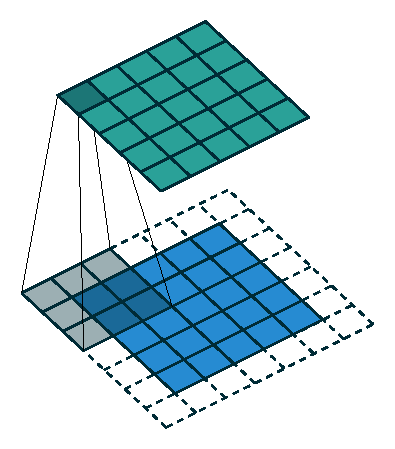
\includegraphics[width=0.23\textwidth]{figures/main/ch2-background/conv_00.pdf}
    \hfill
    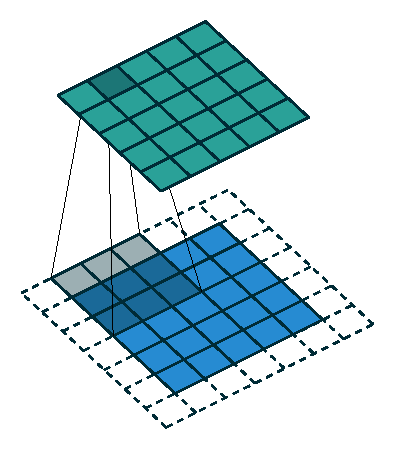
\includegraphics[width=0.23\textwidth]{figures/main/ch2-background/conv_01.pdf}
    \hfill
    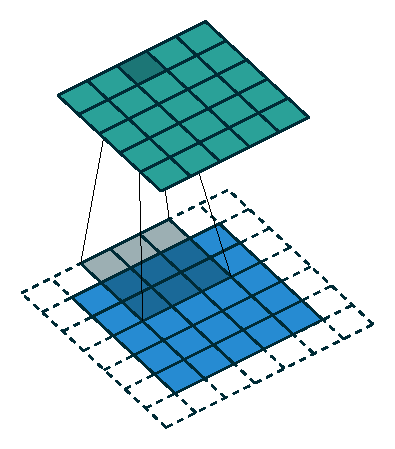
\includegraphics[width=0.23\textwidth]{figures/main/ch2-background/conv_02.pdf}
    \hfill
    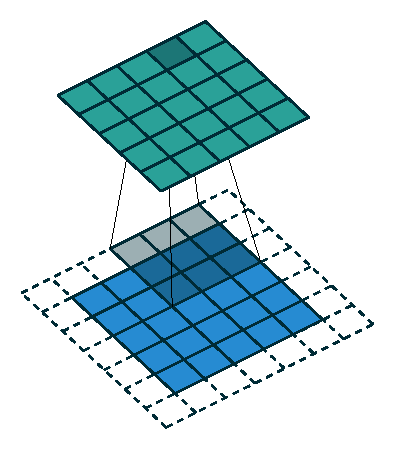
\includegraphics[width=0.23\textwidth]{figures/main/ch2-background/conv_03.pdf}
    \caption{A convolution: a kernel sliding over an image and acting as a filter. \\Illustration taken from~\citet{dumoulin2016guide}}
    \label{figure:illustration_convolution}
\end{figure}

In this subsection, we describe the relation between structured matrices and convolutions.
Recall that a discrete convolution can be seen as a kernel sliding over the image and acting as a filter.
\Cref{figure:illustration_convolution} illustrates the convolution operation with the image (blue), the kernel (gray) and the resulting operation (green).
It has been shown by~\citet{jain1989fundamentals} that the convolution operation is a linear transform `performed' by a doubly-block Toeplitz matrix (in the 2d case), \ie, a block Toeplitz matrix where the blocks are also Toeplitz.
Considering convolutions as a simple linear transformation with a structured matrix has allowed multiple results to be derived~\citet{appuswamy2016structured,wang2020orthogonal,sedghi2018singular,singla2019bounding}, including one of our main contributions presented in \Cref{chapter:ch5-lipschitz_bound}.



% This observation has been made by~\citet{jain1989fundamentals} and many works have been derived from it~\citet{appuswamy2016structured,wang2020orthogonal,sedghi2018singular,singla2019bounding}, including one of our main contributions presented in \Cref{chapter:ch5-lipschitz_bound}.

A discrete convolution operation with a 2-dimensional kernel applied on a 2-dimensional signal is equivalent to a matrix multiplication with a doubly-block Toeplitz matrix.
Let $\Kmat$ be a 2-dimensional kernel defined as follows:
\begin{equation*}
  \Kmat = \leftmatrix
    k_0 & k_1 & k_2 \\
    k_3 & k_4 & k_5 \\
    k_6 & k_7 & k_8 
  \rightmatrix
\end{equation*}
then, the doubly-block Toeplitz matrix $\Mmat$ that performs the convolution can be represented as:
% The doubly-block Toeplitz encoding a convolution parameterized by a 2-dimensional kernel $\Kmat$ can be represented as follows: 
% \begin{equation*}
%   \Mmat = \leftmatrix
%     \Tmat_0 & \Tmat_1 &         &         & 0       \\
%     \Tmat_2 & \Tmat_0 & \Tmat_1 &         &         \\
%             & \Tmat_2 & \ddots  & \ddots  &         \\
%             &         & \ddots  & \Tmat_0 & \Tmat_1 \\
%     0       &         &         & \Tmat_2 & \Tmat_0
%   \rightmatrix
% \end{equation*}
\begin{equation*}
  \Mmat = \leftmatrix
    \Tmat_0 & \Tmat_1 &         &  0       \\
    \Tmat_2 & \Tmat_0 & \ddots  &          \\
            & \ddots  & \Tmat_0 & \Tmat_1  \\
    0       &         & \Tmat_2 &  \Tmat_0
  \rightmatrix
\end{equation*}
where $\Tmat_j$ are banded-Toeplitz matrices and the values of the kernel $\Kmat$ are distributed in the Toeplitz blocks as follows:
% \begin{equation*}
%   \Tmat_0 = \leftmatrixsmall
%     k_4 & k_3 &         &         & 0       \\
%     k_5 & k_4 & k_3 &         &         \\
%             & k_5 & \smallddots  & \smallddots  &         \\
%             &         & \smallddots  & k_4 & k_3 \\
%     0       &         &         & k_5 & k_4
%   \rightmatrixsmall \quad 
%   \hfill
%   \Tmat_1 = \leftmatrixsmall
%     k_7 & k_6 &         &         & 0       \\
%     k_8 & k_7 & k_6 &         &         \\
%             & k_8 & \smallddots  & \smallddots  &         \\
%             &         & \smallddots  & k_7 & k_6 \\
%     0       &         &         & k_8 & k_7 \\
%   \rightmatrixsmall \quad
%   \hfill
%   \Tmat_2 = \leftmatrixsmall
%     k_1 & k_0 &         &         & 0       \\
%     k_2 & k_1 & k_0 &         &         \\
%             & k_2 & \smallddots  & \smallddots  &         \\
%             &         & \smallddots  & k_1 & k_0 \\
%     0       &         &         & k_2 & k_1 \\
%   \rightmatrixsmall
% \end{equation*}
\begin{equation*}
  \Tmat_0 = \leftmatrix
    k_4 & k_3 &         &         & 0       \\
    k_5 & k_4 & k_3 &         &         \\
            & k_5 & \ddots  & \ddots  &         \\
            &         & \ddots  & k_4 & k_3 \\
    0       &         &         & k_5 & k_4
  \rightmatrix \quad 
  \hfill
  \Tmat_1 = \leftmatrix
    k_7 & k_6 &         &         & 0       \\
    k_8 & k_7 & k_6 &         &         \\
            & k_8 & \ddots  & \ddots  &         \\
            &         & \ddots  & k_7 & k_6 \\
    0       &         &         & k_8 & k_7 \\
  \rightmatrix \quad
\end{equation*}

\begin{equation*}
  \Tmat_2 = \leftmatrix
    k_1 & k_0 &         &         & 0       \\
    k_2 & k_1 & k_0 &         &         \\
            & k_2 & \ddots  & \ddots  &         \\
            &         & \ddots  & k_1 & k_0 \\
    0       &         &         & k_2 & k_1 \\
  \rightmatrix
\end{equation*}


However, in practice, the signal can have multiple channel called feature maps (\eg images have 3 channels: RGB).
% corresponding to the colors red, green and blue).
Let us denote by $\cin$ and $\cout$ the number of feature maps of the input and output respectively.
Then the convolution % operation 
takes an input of size $\cin \times n \times n$, is performed by a kernel of size $\cout \times \cin \times k \times k$ and the output signal will be of size $\cout \times m \times m$ with $m = n - k + 2p + 1$ where $p$ corresponds to the padding.
The matrix for the multi-channel convolution is the concatenation of $\cout \cdot \cin$ doubly-block Toeplitz matrices.

